\documentclass[11pt]{article}
\usepackage[margin=1in]{geometry}
\usepackage{amsmath,amssymb,booktabs,graphicx,hyperref}
\graphicspath{{../experiments/manifold_controls_v1/results/}}
\title{Correct Outputs Do Not Make Valid States:\\A Controlled Study of Composable Latent Editing}
\author{Working draft --- authors to be supplied}
\date{October 2026}
\begin{document}
\maketitle
\begin{abstract}
A latent edit can produce the correct text while leaving a state that fails under
the next edit. We study this distinction using a frozen encoder--decoder and
rank-16 affine editors in controlled semantic worlds. History-matched states,
train-fitted low-dimensional interventions, and fresh-world confirmation show
that noncanonical residuals can be hidden from the current output yet cause
continuation failure. In aligned temporal transformations, the same editor class
admits substantially more composable solutions, obtained by closed-form
reduced-rank regression or canonical-state supervision. Cross-entropy refinement
can improve output likelihood while degrading these solutions under AdamW;
optimizer controls qualify this effect. Five-seed confirmation establishes
five-step recovery and a finite closure boundary. A person-domain replication
reproduces the phenomenon but fails to transfer the rank-16 repair. We separate
state validity, finite trajectory success, and robustness, and evaluate
alignment-free manifold and canonical-confidence controls as boundary tests.
\end{abstract}

\section{Introduction}
Editing internal states offers an appealing interface for controlled generation:
an operator changes an attribute and subsequent operators act on its result.
Single-edit evaluation commonly asks whether the decoded output is correct.
That criterion leaves the internal state underdetermined. Two states can decode
to the same text and nevertheless respond differently to an identical future
operator. We call the latter requirement continuation validity.

This paper examines the gap in a controlled setting where the complete target
text and its encoder state are available. Our contribution is an empirical
causal account, rather than a claim of deployment efficiency. We identify
decoder-hidden residuals, establish a composable solution within the same
rank-16 class on one aligned domain, and distinguish objective, optimizer, and
capacity explanations. We preserve negative attribute transfer and finite
closure results as part of the account.

\section{Setting and evaluation}
Let $E$ and $D$ denote the frozen encoder and decoder of BART
\cite{lewis2019bart}. The editable memory has dimension 768 and consists of
masked token states. Each operation is shared across token positions:
\begin{equation}
 T_o(h)=h+U_oV_oh+b_o,\qquad \operatorname{rank}(U_oV_o)\leq16.
\end{equation}
We use finite temporal and grammatical-person states in synthetic worlds with
fixed entities, quantities, colors, and absolute dates. Symbolic operations
provide exact target text $y$. Template 0 is the training format and template 3
is a structural distribution shift. Mask-identical transformations define the
aligned fitting domain. Equal masks are an operational alignment convention,
not a proof of token-level semantic alignment. Length-changing transformations
are reported separately.

For a source $x$ and target $y$, the actual write, canonical write, and residual
are $w=T_o(E(x))-E(x)$, $d=E(y)-E(x)$, and $e=w-d$.
We report single-edit target correctness, non-target preservation, and complete
trajectory success $R_k$: every output through step $k$ must satisfy the target
and preservation checks. We retain exact-text correctness, parseability, and
EOS separately from semantic correctness. Denominators are fixed before
predictions. Wilson intervals describe one trajectory per world; pooled edge
means use world-cluster bootstrap intervals. Seeds remain separate.

Exploratory mechanism worlds were reused across earlier rounds and do not
constitute independent confirmation. A prospectively locked five-seed temporal
confirmation uses 160 new semantic cores excluded from the declared historical
sets. Its mechanism and closure panels use the predetermined first 80 worlds.
The additional person reachability and alignment-free controls have their own
development selection and distinct, prospectively generated confirmation sets.
These three-seed additions remain exploratory method comparisons.

\section{Correct decoding is insufficient for continuation}
Temporal C1 editors achieve complete single-edit correctness on the eight
training-supported transitions in both templates, but their aligned chains
fail at the second edit. History-matched canonical and edited states decode to
the same current text; the canonical state supports continuation while the
edited state fails. Replacing the memory with the target encoding restores
continuation. A separate person-domain experiment reproduces single-edit
success followed by second-step failure on the two supported transformations.
Single-step floors on unsupported templates do not count as composition
evidence.

\section{Mechanism: hidden, direction-specific residuals}
We fit a centered four-dimensional PCA basis $S$ to training-world residuals
and freeze it before evaluating new worlds. Interventions repair the edited
state using the corresponding canonical difference, or inject that difference
into a canonical state. Injection tests both current exact-text preservation
and next-edit failure; repair alone does not establish sufficiency.

Across the new temporal mechanism panel, $S$ and its component orthogonal to the
next editor's reading space restore continuation in every tested eligible
world. Their injections preserve the current exact text and induce next-step
failure. Equal-norm random directions do not produce comparable effects.
Teacher-forced visibility is much smaller before the edit than afterward.
The reading-space component has seed- and template-dependent effects, so the
earlier interpretation that both components are universally necessary does
not survive confirmation. The stronger conclusion is that a low-dimensional
residual outside the next editor's reading space can be causally responsible
for failure through a change in decoder context.

These conclusions concern the chosen intervention and decoding interface.
Reference repair requires a canonical target state. Reference-free coordinate
projection fails and is not presented as a method. Robustness to deliberately
injected residuals is also distinct from suppressing their production.

\section{Cause: canonical writes and output incentives}
\subsection{Reachability within the editor class}
For aligned transitions we solve penalized reduced-rank regression:
\begin{equation}
 \min_{\operatorname{rank}(W)\leq r,b}
 \mathbb E\|E(y)-E(x)-WE(x)-b\|^2+\eta\|W\|_F^2.
\end{equation}
Centered covariance whitening and truncated SVD provide a closed-form
solution. Ridge and rank selection use development worlds only. The temporal
rank-16 solution supports much longer aligned chains than CE-trained editors.
An L2-trained editor also reaches a composable solution, arguing against
capacity, data coverage, or inability of gradient training as the principal
explanation on this domain. Full-rank L2 failure would not establish that no
decoder-relevant linear solution exists: unweighted state MSE is a surrogate.

\subsection{Writing geometry}
Historical CE writes are nearly orthogonal to canonical writes. Across three
seeds on IID aligned transitions, $\cos(w,d)$ is between $-0.0119$ and
$-0.0052$, while $\|w\|/\|d\|$ is 3.31--3.40; the structural-shift ratios
are 3.69--3.80. Thus the write is substantial relative to the ideal semantic
change while contributing almost no positive movement along its direction.
These results support a decoder-directed shortcut interpretation, connecting
conceptually to shortcut learning \cite{geirhos2020shortcut}. They do not prove
an adversarial attack \cite{szegedy2013intriguing}, nor that the write is large
relative to the entire source representation.

\subsection{Canonical states need not minimize output CE}
Paired teacher-forced comparisons show that edited states can assign greater
likelihood to the same target than $E(y)$ itself. Hence canonical encoding is
not a minimum of the finite-panel output objective. Absolute improvements are
small in nats per token despite large percentage reductions.

C4 initializes the rank-16 editor at the canonical RRR solution and refines it
with CE. Under AdamW at learning rate $10^{-3}$, single-edit correctness
persists while residuals grow and five-step success collapses. Pure SGD and
smaller AdamW learning rates also reduce CE, but preserve substantially more
composition at the measured checkpoints. Therefore CE can reward noncanonical
writes, while the degree of continuation damage depends on optimizer and
trajectory. We do not claim that every CE optimizer must destroy composition.
The hidden-state CE descent direction at RRR initialization has almost zero
cosine with the ideal write. Hidden gradients are not identical to updates of
shared low-rank factors.

\begin{figure}[t]
\centering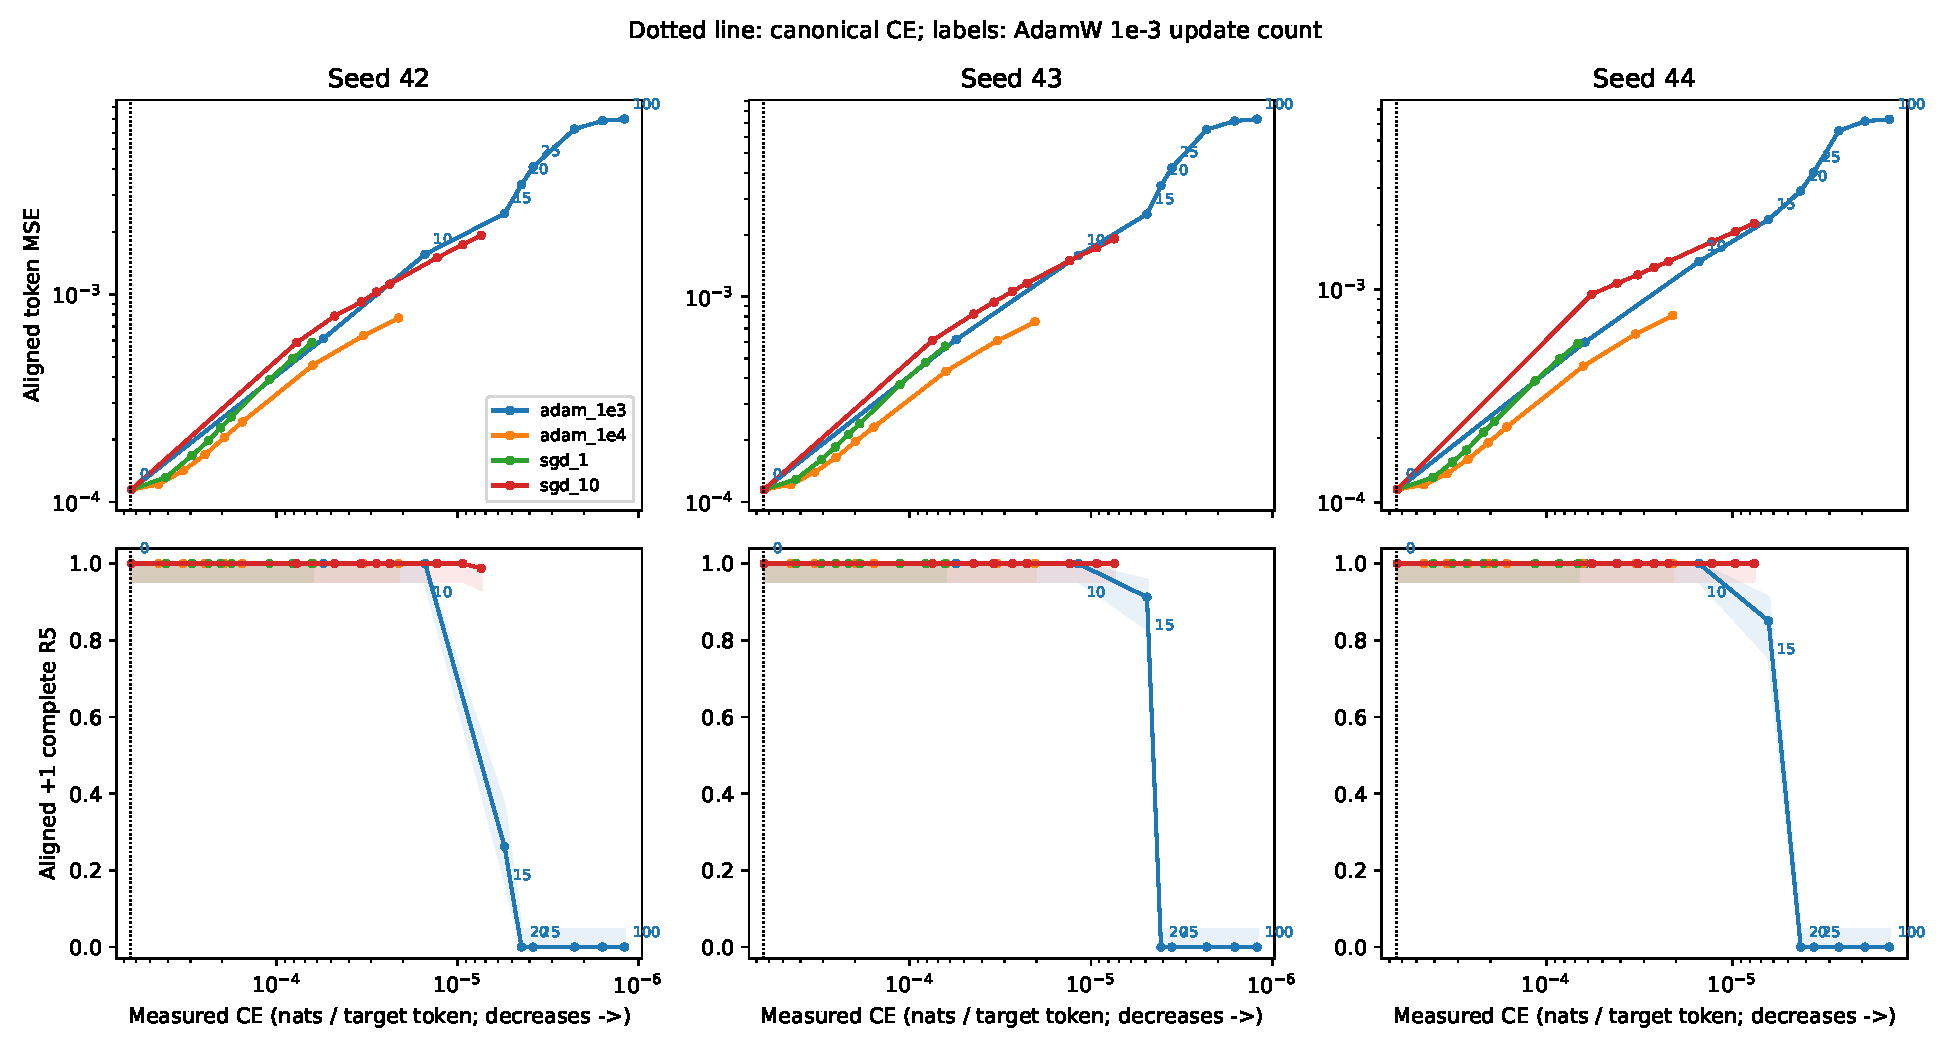
\includegraphics[width=\linewidth]{optimizer_absolute_ce.pdf}
\caption{Measured optimizer checkpoints, indexed by absolute target-token CE.
The dotted reference marks canonical CE. Residual uncertainty is bootstrapped
by world; $R_5$ intervals are Wilson intervals. Labels show update counts.
Connecting lines do not constitute measurements of intermediate models.}
\end{figure}

\section{Repair and its boundaries}
Canonical anchoring adds normalized aligned-state MSE to CE:
\begin{equation}
 \mathcal L_{\mathrm{canon}}=\mathrm{CE}(D(T_o(E(x))),y)
 +\lambda\frac{\|T_o(E(x))-\operatorname{sg}[E(y)]\|^2_{\mathrm{valid}}}
 {n\,768\,\sigma_o^2},
\end{equation}
where $\sigma_o^2$ is the training-only per-token ideal-write energy and
$\lambda=1$ in the fixed comparison. No canonical test states enter training.
In the locked
five-seed temporal confirmation, C3 attains 100\% complete five-step success
on aligned paths in both templates. It also preserves every trajectory through
20 steps on the closure panel, but 50-step success varies from 0\% to 100\%
with seed, cycle, and template. Affine cycle spectra and measured residual
growth diagnose this boundary; spectral radius greater than one does not imply
that every initial state excites an unstable direction.

Scalar residual amplitude predicts risk within panels but does not define a
shared calibrated threshold across editor families. Higher-MSE states can
support continuation where lower-MSE states fail. Residual direction and the
future operator matter. Earlier third-step supervision and one-step KL
lookahead provide different empirical horizons; these finite experiments do
not establish a universal ceiling for trajectory objectives.

The rank-16 person-domain repair does not transfer: residuals decrease but
second-step success remains zero. Its inherited-ridge RRR initialization also
fails the single-step admission check. We therefore diagnose reachability
using a development-selected rank curve before interpreting this outcome as
an objective or capacity failure. That follow-up selects rank 256 on dev;
on 160 separate worlds its supported single-edit mean is 30.31\% and forward
and reverse complete $R_5$ are 12.50\% and 11.25\%. Full rank reduces aligned
MSE further but still fails admission and general repair. These results rule
out a simple ``raise the rank'' fix under this fitted L2 objective, not the
existence of every possible decoder-relevant linear solution.

\subsection{Alignment-free controls}
Emb2Emb constrains mapped embeddings using a discriminator over encoder
representations \cite{mai2020emb2emb}. We adapt this idea to masked token
memory with CE task supervision, a pooled-mean discriminator, and a token-set
sensitivity control. This is not a reproduction of the original supervised
cosine-embedding objective. Genuine real states are sampled from canonical
training sequences matched to the edited source length, eliminating trivial
padding cues. The constraint concerns the marginal accessible state
distribution, not a paired canonical target. We select three regularization
weights on development data and report discriminator generalization along
with composition; finite discriminator failure cannot refute all manifold
regularization.

Both selected discriminator variants preserve 98.12--100\% single-edit success
across seeds and templates, while forward aligned $R_5$ remains zero.
Held-out dev discriminators still separate real and fake distributions
(AUROC 0.798--1.000). Thus this finite-budget adaptation does not repair
composition and has not established empirical state-distribution matching.
It is not direct evidence of a genuinely on-manifold but noncanonical state;
sampling priors, the length interface, discriminator capacity, and adversarial
optimization remain possible explanations.

We also test the canonical-confidence floor
\begin{equation}
 \mathcal L_{\mathrm{floor}}=
 \mathbb E\max\{\mathrm{CE}(D(T_o(E(x))),y)
 -\operatorname{sg}[\mathrm{CE}(D(E(y)),y)],0\}.
\end{equation}
The hinge is applied per example before averaging and requires no token
alignment. Unlike conventional flooding \cite{ishida2020flooding}, it stops the
loss gradient below the floor rather than reversing it. Adam momentum may
still move parameters there, as can updates for other examples through shared
parameters. The new-world floor comparison preserves 100\% single-edit success
for all three seeds in both templates, while forward aligned $R_5$ remains
0\%. Residual MSE decreases only slightly relative to coverage-matched CE.
Removing this additional likelihood incentive alone therefore does not select
valid states under the tested objective and optimizer setting.

\paragraph{Follow-up status.}
The development-selected person rank curve and alignment-free controls are
being evaluated under a separate locked protocol. Numerical results will be
inserted from the checked confirmation summaries. No outcome is assumed here.


\section{Limitations and scope}
The causal evidence comes from a frozen BART interface and synthetic worlds.
Template shift and attribute replication do not substitute for independent
model-family replication or natural text. We have not solved length-changing
canonicalization, guaranteed arbitrary-length closure, or protected against
targeted latent perturbations. Decoder-only temporal replication remains
future work pending a specified state layer and read/write interface; it must
begin with reconstruction admission and oracle repair before testing
phenomenon, C1/C3/C4, and difference-of-means steering. Re-encoding is an
empirical canonical reference with modest measured cost; computational savings
are not the main motivation for this work.

\begin{thebibliography}{9}
\bibitem{lewis2019bart} Mike Lewis et al. 2019.
BART: Denoising Sequence-to-Sequence Pre-training for Natural Language
Generation, Translation, and Comprehension. \href{https://arxiv.org/abs/1910.13461}{arXiv:1910.13461}.
\bibitem{mai2020emb2emb} Florian Mai, Nikolaos Pappas, Ivan Montero,
Noah A. Smith, and James Henderson. 2020.
Plug and Play Autoencoders for Conditional Text Generation. EMNLP.
\href{https://aclanthology.org/2020.emnlp-main.491/}{ACL Anthology}.
\bibitem{geirhos2020shortcut} Robert Geirhos et al. 2020.
Shortcut Learning in Deep Neural Networks.
\href{https://arxiv.org/abs/2004.07780}{arXiv:2004.07780}.
\bibitem{szegedy2013intriguing} Christian Szegedy et al. 2013.
Intriguing properties of neural networks.
\href{https://arxiv.org/abs/1312.6199}{arXiv:1312.6199}.
\bibitem{ishida2020flooding} Takashi Ishida et al. 2020.
Do We Need Zero Training Loss After Achieving Zero Training Error?
\href{https://arxiv.org/abs/2002.08709}{arXiv:2002.08709}.
\end{thebibliography}
\end{document}
